\section{Finite Automata}

Finite automata adalah model matematika yang digunakan untuk mengenali string dalam suatu bahasa. Terdapat dua jenis utama: NFA (Nondeterministic Finite Automata) dan DFA (Deterministic Finite Automata).

\subsection{Definisi Formal}

\textbf{Finite Automaton} didefinisikan sebagai tuple $(Q, \Sigma, \delta, q_0, F)$ dimana:
\begin{itemize}
    \item $Q$: Himpunan state (keadaan) yang terbatas
    \item $\Sigma$: Alphabet (himpunan simbol input)
    \item $\delta$: Fungsi transisi (transition function)
    \item $q_0$: Start state (state awal)
    \item $F$: Himpunan accept states (final states)
\end{itemize}

\subsection{NFA (Nondeterministic Finite Automata)}

NFA memiliki karakteristik:
\begin{itemize}
    \item Untuk suatu state dan input symbol, dapat memiliki \textbf{nol, satu, atau lebih} transisi
    \item Dapat memiliki \textbf{$\epsilon$-transitions} (epsilon transitions) yang tidak mengonsumsi input
    \item Lebih mudah dikonstruksi dari regular expression
    \item Simulasi memerlukan backtracking atau multiple states tracking
\end{itemize}

Contoh NFA untuk pattern \texttt{a|b}:

Gambar \ref{fig:nfa-union} menunjukkan NFA untuk pattern \texttt{a|b} yang menggunakan $\epsilon$-transitions untuk branching.

\begin{figure}[!htbp]
    \centering
    \adjustbox{max width=0.7\textwidth,center}{%
    \begin{tikzpicture}[
        state/.style={circle, draw=blue!50, fill=blue!10, minimum size=0.8cm, font=\footnotesize},
        accept/.style={circle, draw=green!50, fill=green!10, minimum size=0.8cm, font=\footnotesize, double},
        start/.style={circle, draw=red!50, fill=red!10, minimum size=0.8cm, font=\footnotesize},
        arrow/.style={->, >=stealth, thick},
        eps/.style={->, >=stealth, thick, dashed, blue!70},
        node distance=1.5cm and 2cm
    ]
    
    % Start state
    \node[start] (q0) at (0,0) {$q_0$};
    
    % Accept states
    \node[accept] (q1) at (-2,-2) {$q_1$};
    \node[accept] (q2) at (2,-2) {$q_2$};
    
    % Epsilon transitions
    \draw[eps] (q0) to[out=225, in=90] node[left, font=\tiny] {$\epsilon$} (q1);
    \draw[eps] (q0) to[out=315, in=90] node[right, font=\tiny] {$\epsilon$} (q2);
    
    % Symbol transitions
    \draw[arrow] (q1) to[loop left] node[left, font=\tiny] {$a$} (q1);
    \draw[arrow] (q2) to[loop right] node[right, font=\tiny] {$b$} (q2);
    
    % Labels
    \node[above=0.2cm of q0, font=\small] {\textbf{Start}};
    \node[below=0.2cm of q1, font=\tiny] {\textbf{Accept}};
    \node[below=0.2cm of q2, font=\tiny] {\textbf{Accept}};
    
    \end{tikzpicture}%
    }
    \caption{NFA untuk pattern \texttt{a|b} dengan $\epsilon$-transitions}
    \label{fig:nfa-union}
\end{figure}

State $q_0$ adalah start state, $q_1$ dan $q_2$ adalah accept states. Dari $q_0$, dengan $\epsilon$-transition dapat menuju $q_1$ atau $q_2$, kemudian dari $q_1$ dapat menerima 'a', dan dari $q_2$ dapat menerima 'b'.

\subsection{DFA (Deterministic Finite Automata)}

DFA memiliki karakteristik:
\begin{itemize}
    \item Untuk setiap state dan input symbol, terdapat \textbf{tepat satu} transisi
    \item Tidak memiliki $\epsilon$-transitions
    \item Lebih efisien untuk simulasi (deterministic)
    \item Setiap NFA dapat dikonversi menjadi DFA yang ekuivalen
\end{itemize}

Contoh DFA untuk pattern \texttt{a|b}:

Gambar \ref{fig:dfa-union} menunjukkan DFA yang ekuivalen dengan NFA di atas, tetapi deterministik.

\begin{figure}[!htbp]
    \centering
    \adjustbox{max width=0.6\textwidth,center}{%
    \begin{tikzpicture}[
        state/.style={circle, draw=blue!50, fill=blue!10, minimum size=0.8cm, font=\footnotesize},
        accept/.style={circle, draw=green!50, fill=green!10, minimum size=0.8cm, font=\footnotesize, double},
        start/.style={circle, draw=red!50, fill=red!10, minimum size=0.8cm, font=\footnotesize},
        arrow/.style={->, >=stealth, thick},
        node distance=2cm
    ]
    
    % Start state
    \node[start] (q0) at (0,0) {$q_0$};
    
    % Accept states
    \node[accept] (q1) at (-2,-2) {$q_1$};
    \node[accept] (q2) at (2,-2) {$q_2$};
    
    % Transitions
    \draw[arrow] (q0) to[out=225, in=90] node[left, font=\tiny] {$a$} (q1);
    \draw[arrow] (q0) to[out=315, in=90] node[right, font=\tiny] {$b$} (q2);
    
    % Self loops
    \draw[arrow] (q1) to[loop left] node[left, font=\tiny] {$a$} (q1);
    \draw[arrow] (q2) to[loop right] node[right, font=\tiny] {$b$} (q2);
    
    % Labels
    \node[above=0.2cm of q0, font=\small] {\textbf{Start}};
    \node[below=0.2cm of q1, font=\tiny] {\textbf{Accept}};
    \node[below=0.2cm of q2, font=\tiny] {\textbf{Accept}};
    
    \end{tikzpicture}%
    }
    \caption{DFA untuk pattern \texttt{a|b} (deterministik)}
    \label{fig:dfa-union}
\end{figure}

DFA ini deterministik: dari $q_0$, input 'a' selalu menuju $q_1$, input 'b' selalu menuju $q_2$. Tidak ada $\epsilon$-transitions dan setiap state memiliki tepat satu transisi untuk setiap input symbol.

\subsection{Perbedaan NFA dan DFA}

Perbedaan utama antara NFA dan DFA dapat dilihat pada Tabel \ref{tab:nfa-dfa} dan perbandingan visual pada Gambar \ref{fig:nfa-dfa-comparison}.

\begin{table}[!htbp]
\centering
\begin{tabularx}{\textwidth}{|l|X|X|}
\hline
\textbf{Aspek} & \textbf{NFA} & \textbf{DFA} \\
\hline
Transisi per state & Bisa 0, 1, atau lebih & Tepat 1 \\
\hline
$\epsilon$-transitions & Diizinkan & Tidak diizinkan \\
\hline
Efisiensi simulasi & Perlu backtracking & Linear time \\
\hline
Jumlah states & Biasanya lebih sedikit & Bisa lebih banyak \\
\hline
Konstruksi dari regex & Lebih mudah & Lebih kompleks \\
\hline
\end{tabularx}
\caption{Perbandingan NFA dan DFA}
\label{tab:nfa-dfa}
\end{table}

\begin{figure}[!htbp]
    \centering
    \adjustbox{max width=0.9\textwidth,center}{%
    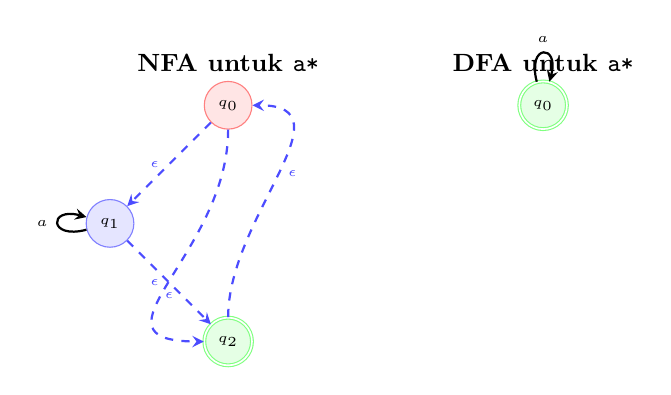
\begin{tikzpicture}[
        state/.style={circle, draw=blue!50, fill=blue!10, minimum size=0.6cm, font=\tiny},
        accept/.style={circle, draw=green!50, fill=green!10, minimum size=0.6cm, font=\tiny, double},
        start/.style={circle, draw=red!50, fill=red!10, minimum size=0.6cm, font=\tiny},
        arrow/.style={->, >=stealth, thick},
        eps/.style={->, >=stealth, thick, dashed, blue!70},
        node distance=1.2cm
    ]
    
    % NFA side
    \node[font=\small\bfseries, above=0.3cm] at (-2,0) {NFA untuk \texttt{a*}};
    \node[start] (nq0) at (-2,0) {$q_0$};
    \node[state] (nq1) at (-3.5,-1.5) {$q_1$};
    \node[accept] (nq2) at (-2,-3) {$q_2$};
    
    \draw[eps] (nq0) -- node[left, font=\tiny] {$\epsilon$} (nq1);
    \draw[arrow] (nq1) to[loop left] node[left, font=\tiny] {$a$} (nq1);
    \draw[eps] (nq1) -- node[left, font=\tiny] {$\epsilon$} (nq2);
    \draw[eps] (nq0) to[out=270, in=180, looseness=1.5] node[below, font=\tiny] {$\epsilon$} (nq2);
    \draw[eps] (nq2) to[out=90, in=0, looseness=1.2] node[right, font=\tiny] {$\epsilon$} (nq0);
    
    % DFA side
    \node[font=\small\bfseries, above=0.3cm] at (2,0) {DFA untuk \texttt{a*}};
    \node[start,accept] (dq0) at (2,0) {$q_0$};
    
    \draw[arrow] (dq0) to[loop above] node[above, font=\tiny] {$a$} (dq0);
    
    \end{tikzpicture}%
    }
    \caption{Perbandingan visual NFA dan DFA untuk pattern \texttt{a*} (keduanya ekuivalen)}
    \label{fig:nfa-dfa-comparison}
\end{figure}